\documentclass{supervision}
\usepackage{course}

\Supervision{1}

\begin{document}
  \begin{questions}
    \question Write a 300-word description of what NFS is, how it works, and
      when you might use it and why. Please read around the subject a bit. No
      cut-n-paste from other resources!

    \section*{2010 Paper 5 Question 6}
    \question
      \begin{parts}
        \part[10] When distributed systems are designed and engineered, certain
          fundamental characteristics have to be taken into account, including:

          \begin{enumerate}
            \item Concurrent execution of components.
            \item Independent failure modes
            \item Communication delay
            \item No gobal time
          \end{enumerate}

          In the light of these characteristics, discuss the monitoring of a
          widely distributed industrial process with the following properties:

          Distributed monitoring computers analyse regions of the process. Each
          region contains a number of sensors at identified locations and with
          the ability to generate timestamps. Some sensors monitor temperature,
          others monitor pressure.


          If both temperature and pressure are found by a monitoring computer
          to be above their defined thresholds in a given locality within its
          region it sends an alarm signal to the process control centre,
          indicating the time and place of the occurrence. The control centre
          initiates action to bring the values under control.

        \part[10] The diagram below represents a process group that
          communicates by means of multicast messages.

          \begin{center}
            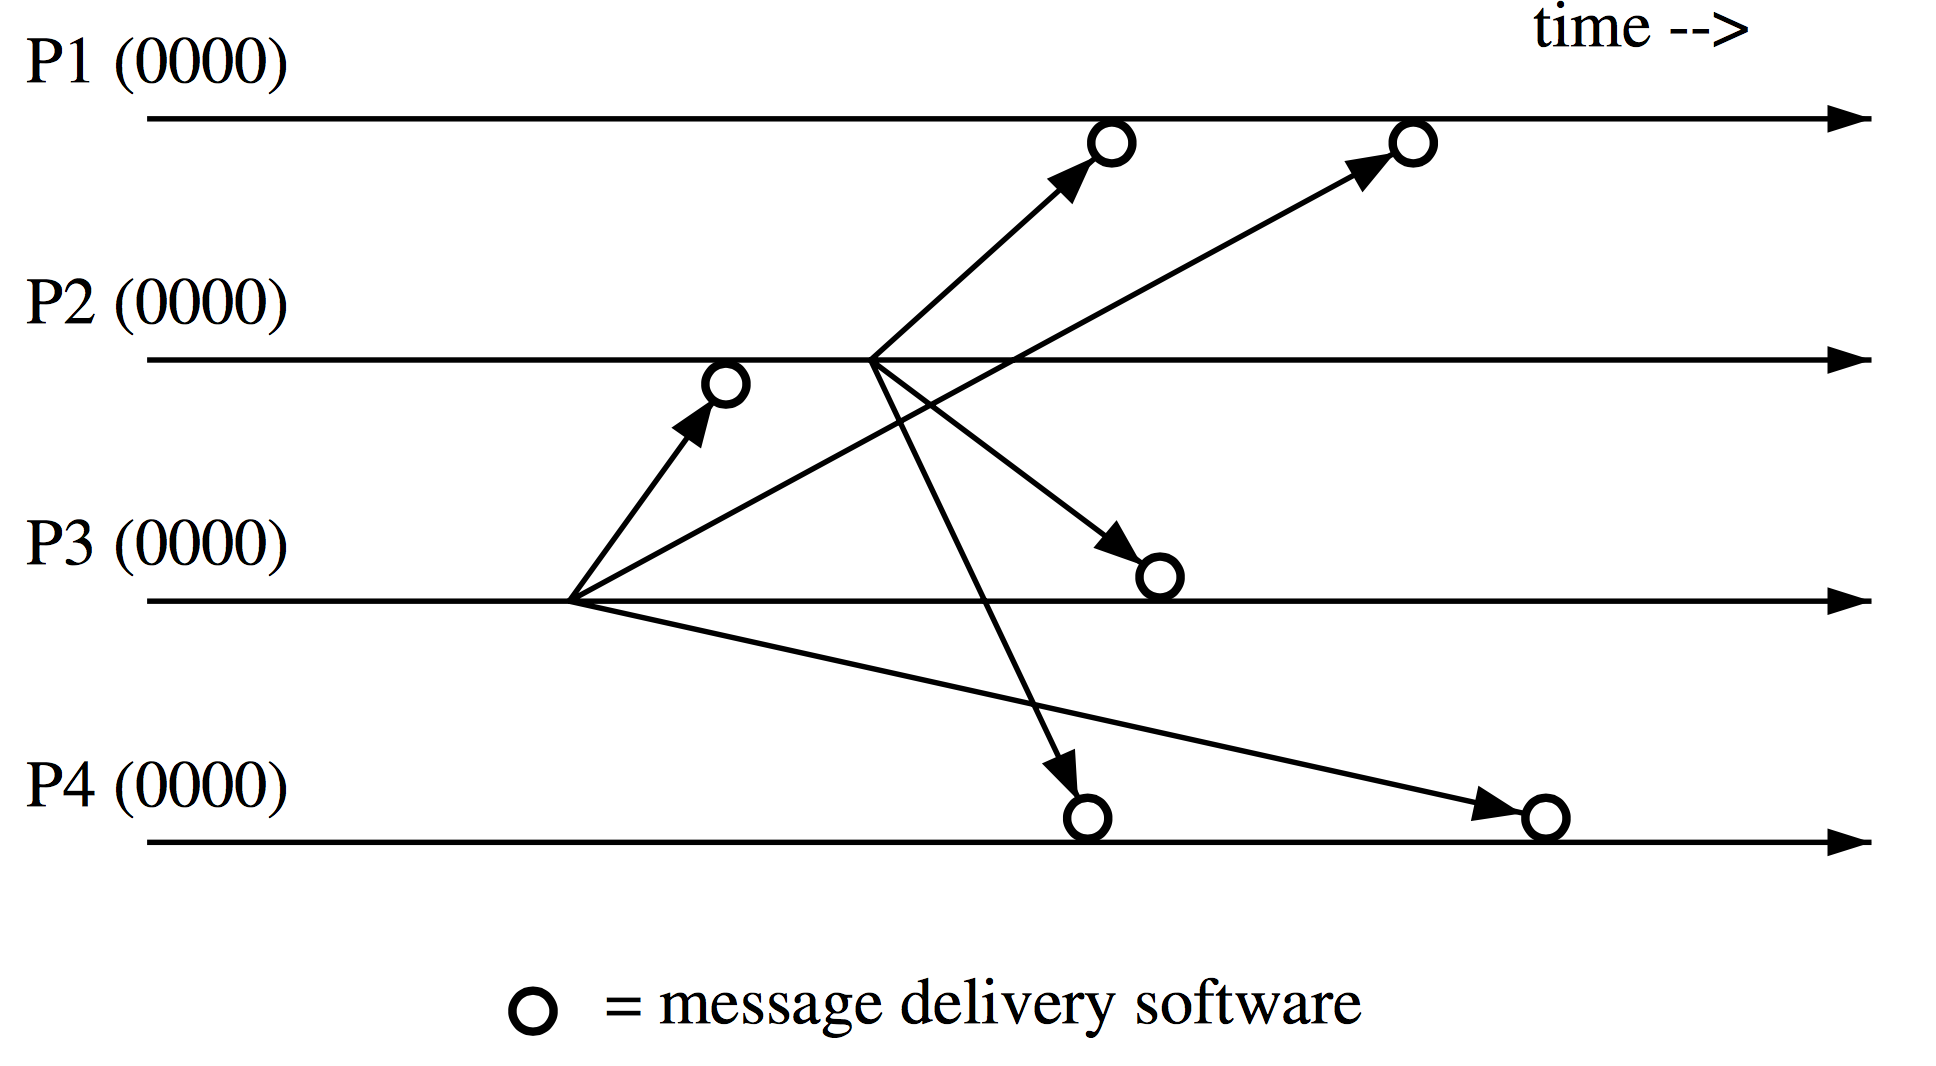
\includegraphics[width=0.75\textwidth]{2010-p5-q6-diagram}
          \end{center}

          At each process-hosting node, message delivery software decides
          whether an incoming message should be delivered to the process or
          buffered for later delivery. This is achieved by the use of vector
          clocks.

          With reference to the example shown in the diagram, describe the
          vector clock algorithm for delivery of messages in causal order.

      \end{parts}

    \section*{2011 Paper 5 Question 9}
    \question
      \begin{parts}
        \part We have considered four types of middleware: remote procedure
          call, object-oriented middleware, message-oriented middleware, and
          event-based middleware.

          \begin{subparts}
            \subpart[4] Each middleware has a core action, such as a remote
              procedure call or a remote method invocation. This entails data
              transfer that is either unidirectional (out of or into the
              calling context) or bidirectional (in and out). State which is
              used by each of the four types of middleware.

            \subpart[2] Does each of these; uni and bidirectional data
              transfer have sufficient expressive power for programming?
              Explain your answer.

            \subpart[4] One of the characteristics of distributed systems is
              that they lack global time. Given your answers above, what
              effect might this have on middleware use?

          \end{subparts}
        \part
          \begin{subparts}
            \subpart[2] What are causal and totally ordered message delivery?

            \subpart[1] Which does vector clocks provide?

            \subpart[2] The vector clock algorithm is a way of sharing state,
              ensuring that every process knows what it needs to about how far
              the others have progressed. Why is it critical that messages
              having vector timestamps are never lost?

          \end{subparts}
        \part
          \begin{subparts}
            \subpart[2] Storage services can be \emph{stateful} or
              \emph{stateless}. Give \textbf{one} advantage and \textbf{one}
              disadvantage of each.

            \subpart[3] If you were designing a service to support film
              production, which would you use and why?

          \end{subparts}
      \end{parts}

    \section*{Practical Programming}
    \question Write a Java program which acts as an NTP client and prints the
      current time, as estimated from the NTP server, to the console whenever
      it is run. For example:

      \begin{code}{sh}
        bash $ java -jar current-time.jar
        Fri Feb 24 15:24:54 GMT 2012
        bash $
      \end{code}

      You will need to send UDP packets in an appropriate format to an NTP
      server. The Computer Lab has a set of NTP servers which you may wish to
      use:

      \begin{code}{}
        server ntp0.cl.cam.ac.uk
        server ntp1a.cl.cam.ac.uk
        server ntp1b.cl.cam.ac.uk
        server ntp1c.cl.cam.ac.uk
        server ntp1d.cl.cam.ac.uk
      \end{code}

      Please make sure your packets conform to NTP version 3 or later (see RFC
      1305 or later) and that you don't send more than two packets to the
      server each time you run your program.
  \end{questions}
\end{document}
